\section{Experiment 10H-L: validation-selected fits and global fallback}
\label{sec:experiment10hl}

\paragraph{Question and fixed design.}
Experiment 10H-K establishes an average future-output benefit from two jointly
learned plants, with unfavorable client outcomes and competing stationary
solutions. Experiment 10H-L tests whether client-blocked validation can select
a reproducible fitting strategy and whether causal calibration can support
group choice with a global fallback. Protocol commit \texttt{6cc2ad0} precedes
execution; every fitting manifest records implementation \texttt{d744941}.
Fleets 601--605 and their outer clients remain opened development evidence.
Confirmation seeds 591--600 and 611--620 remain sealed.

The measured arrays, 20 training/ten outer clients per fleet, eight-coordinate
coupling, coefficient multiplier box $[0.1,10]$, public $R$, fixed $Q$ shape
and scales 0.01/1, bias correction and numerical limits are unchanged.
Neither bounds nor covariance panels are selected here. Two inner folds
block all speed records of each training client together: sorted client rank
modulo two assigns ten fitting and ten validation clients to each fold.
Each inner global plant uses three starts; each two-plant fit uses six.
All contexts share six deterministic split directions around their own learned
global plant. On the full 20-client training set, the archived global fit and
first three mixture starts are audited and reused; only three additional
mixture starts are fitted. A direction is eligible only when both inner fits
and its full fit pass success, KKT and feasibility checks.

\paragraph{Causal decision and selection rules.}
Each validation or outer client supplies the first 100 samples (1\,s) of its
first listed record. Each of the global and two group plants scores fixed-$R$
forecasts at horizons 5, 20 and 50 samples, using common prefix origins
20--50 inclusive. Every forecast filters strictly earlier measurements and
then propagates commands without intervening output corrections. The mean
three-horizon error is the candidate's calibration score. The group with the
smaller score is deployed only if its score is strictly below
$(1-\delta)$ times the global score; otherwise the client retains the global
plant. The predeclared margins are $\delta\in\{0,0.1,0.25\}$.
One choice is frozen across all that client's subsequent speed records.

For every restart direction and margin, inner validation assesses future
outputs at horizons 5, 20 and 50 from origins 100--150 inclusive. Its selection
score averages $\log(E_{ig,h}/E_{i,\mathrm{global},h})$ equally across clients,
horizons and folds. Only this inner score selects direction and margin;
ties within $10^{-12}$ prefer a larger margin, then a lower restart index.
The full fit transfers the selected initialization direction, which does not
identify an invariant optimizer basin across training subsets.

Outer comparisons include the global plant, six-start training-likelihood
winner with prefix likelihood MAP, validation-selected fit with the same MAP,
that selected fit with forecast group choice, and the primary forecast choice
with fallback. The archived three-start winner and public nominal plant are
also retained. All seven methods have the same 100-sample calibration budget,
forecast origins 100--150 and horizons 1, 5, 20 and 50. Zero-start simulations
propagate from the record start but score samples 100--199. These windows
differ from 10H-K's 50-sample calibration and are compared only within 10H-L.

\paragraph{Numerical execution and independent audit.}
All 250 fit records pass success and stationarity/feasibility checks: 210 new
fits and 40 archived fits. Maximum KKT residual is $1.95\times10^{-5}$,
maximum constraint violation $6.30\times10^{-13}$, and maximum physical
coupling residual $1.78\times10^{-15}$. There are no invalid fitting
evaluations. All six strategies are numerically eligible in every fleet/panel.
Selection chooses a 25\% margin in eight jobs and zero in two; no 10\%
margin is selected. Numerical convergence therefore does not explain the
adverse validation transfer described below.

The independent reporting audit verifies ten job manifests, 30 context caches,
committed source hashes, all measured arrays and whole-client fold isolation.
Aggregate tables reproduce the verified individual jobs exactly. Saved inner
scores reproduce selection without outer information. The earlier independent
single-model evaluator reproduces first-record calibration scores to
$9.38\times10^{-12}$, frozen-choice future errors to $2.04\times10^{-12}$
and zero-start suffix errors to $2.12\times10^{-12}$. Historical 10H-I/J/K
gate artifacts remain byte-identical. Six additional tests cover prefix
isolation, causal propagation, forecast equivalence, strict fallback decisions,
inner selection/eligibility and the sealed-seed configuration. The full suite
passes 142 tests, and all four new Python files pass scoped lint.

\paragraph{Mixed future-output result.}
Table~\ref{tab:10hl-selection} separates fitting-strategy choice from client
assignment. At $Q=0.01$, the primary rule reduces mean 0.5\,s error from
49.081 for six-start likelihood MAP to 37.357; its mean paired fleet gain
is 22.24\%, with improvement in every fleet. The primary gain relative to
the global plant is 76.64\%. At $Q=1$, mean error instead rises from 56.430
to 87.738; mean paired gain is $-60.19\%$, with deterioration in every fleet
relative to likelihood MAP. The primary still improves the global plant in
every fleet, with mean paired gain 59.60\%. Positive global-relative gain
alone would conceal the failed improvement over the available mixture baseline.

\begin{table}[htbp]
\centering
\caption{Outer 0.5\,s fixed-$R$ output errors, averaged across five fleets.
The final column averages paired fleet reductions relative to the six-start
likelihood-MAP rule. Calibration and future windows are identical for all rows.}
\label{tab:10hl-selection}
\begin{tabular}{llrr}
\toprule
$Q$ scale & Deployment & Mean $E_R$ & Gain vs likelihood MAP (\%)\\
\midrule
0.01 & Global & 161.187 & ---\\
0.01 & Archived three-start MAP & 47.320 & 2.47\\
0.01 & Six-start likelihood MAP & 49.081 & 0.00\\
0.01 & Validation fit + MAP & 46.606 & 6.82\\
0.01 & Validation fit + forecast group & 46.580 & 6.59\\
0.01 & Validation fit + fallback & 37.357 & 22.24\\
\midrule
1 & Global & 221.235 & ---\\
1 & Archived three-start MAP & 58.452 & $-3.87$\\
1 & Six-start likelihood MAP & 56.430 & 0.00\\
1 & Validation fit + MAP & 87.279 & $-58.88$\\
1 & Validation fit + forecast group & 104.405 & $-91.70$\\
1 & Validation fit + fallback & 87.738 & $-60.19$\\
\bottomrule
\end{tabular}
\end{table}

The horizon/simulation results agree with this split. At $Q=0.01$, primary
one-step and 0.2\,s errors fall from 3.100/42.256 to 2.883/31.143, and
suffix simulation from 47.019 to 35.971. At $Q=1$, the corresponding errors
rise from 1.809/32.900 to 1.825/42.970 and simulation from 66.296 to 110.070.
Both fixed covariance panels and every predeclared ablation remain visible
in the saved tables and Figure~\ref{fig:10hl-selection}.

\begin{figure}[htbp]
\centering
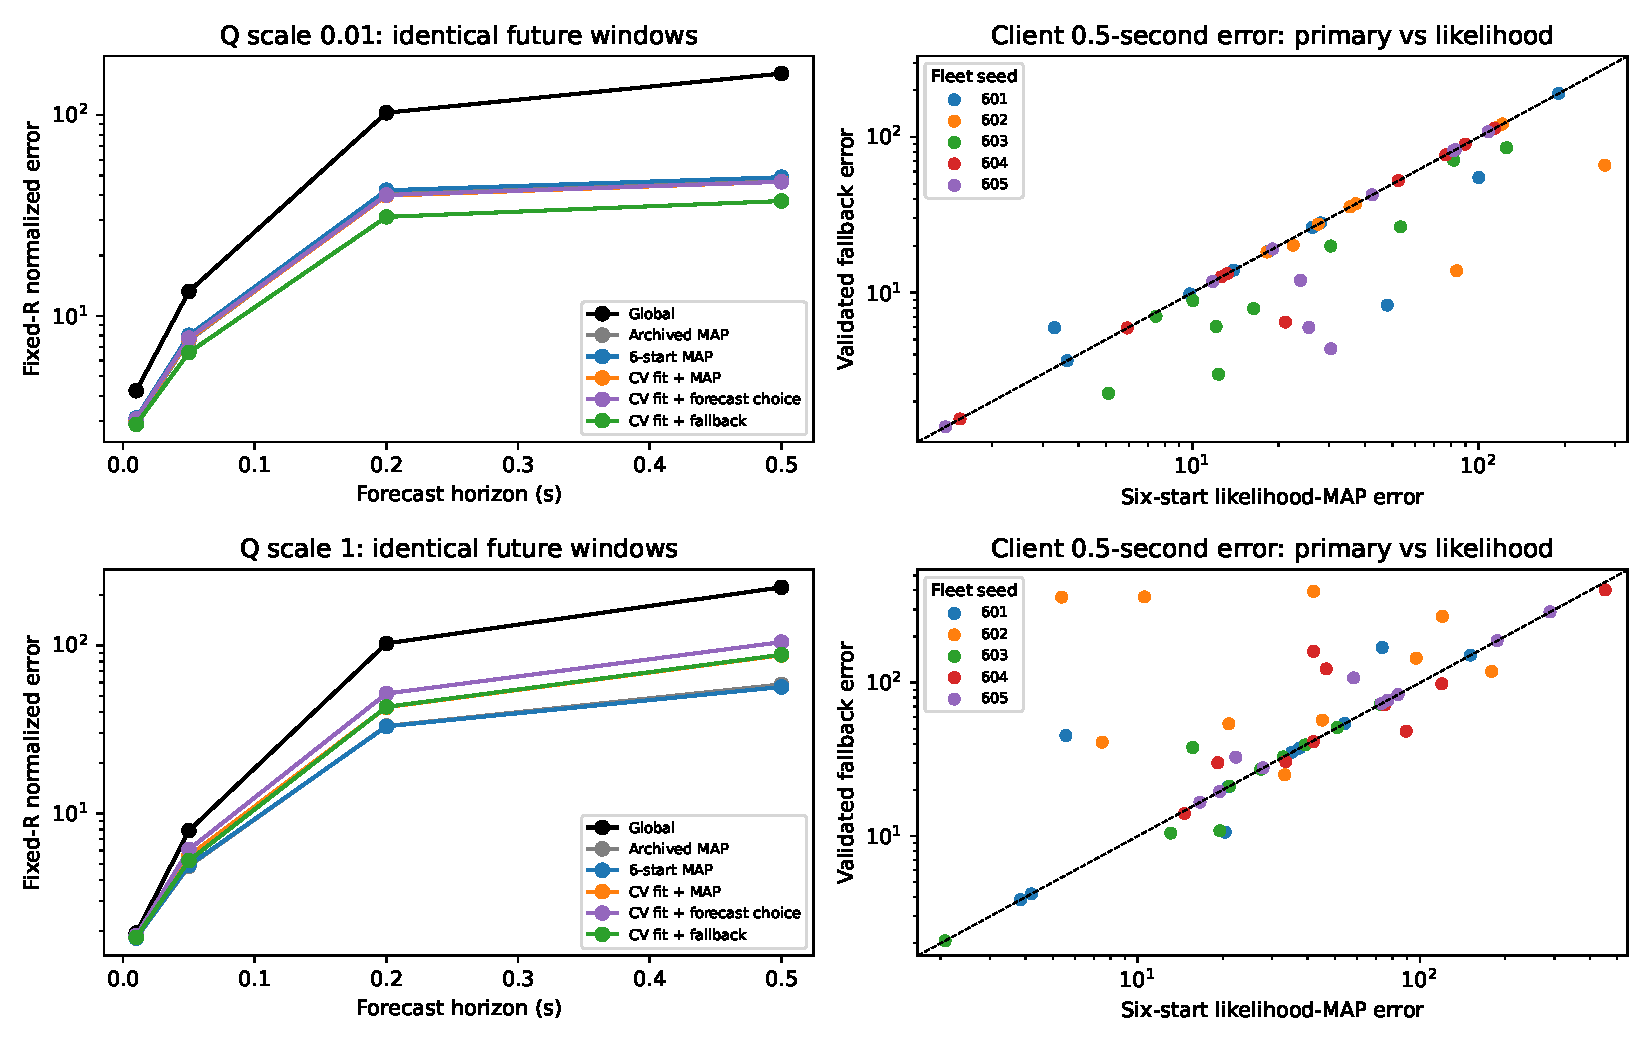
\includegraphics[width=\textwidth]{../results/figures/experiment_10hl_validated_selection.pdf}
\caption{Left: mean future errors on common post-calibration origins.
Right: individual-client 0.5\,s errors of the primary rule against six-start
likelihood MAP. Points above the identity line deteriorate. Colors identify
fleet seeds, without vehicle class labels.}
\label{fig:10hl-selection}
\end{figure}

\paragraph{Fallback reduces global-relative losses but supplies no guarantee.}
At $Q=0.01$, likelihood MAP improves 37/50 clients and degrades 13/50
relative to the global plant. The primary improves 36, leaves 13 unchanged
through global fallback, and degrades one. Its worst global-relative error
ratio falls from 6.98 to 1.73. At $Q=1$, likelihood MAP improves 42 and
degrades eight; the primary improves 31, leaves 16 unchanged, and degrades
three. The worst ratio falls only from 2.19 to 2.13.

Absolute error tails give a further qualification. At $Q=0.01$, the
likelihood/primary 90th-percentile client errors are 113.67/108.00 and maxima
275.79/190.48. At $Q=1$, maxima fall from 453.67 to 402.03, while the
90th percentile rises from 123.21 to 272.34 and median from 36.36 to 46.72.
Against likelihood MAP, the worst primary client error ratio is 1.80 at
$Q=0.01$ and 67.16 at $Q=1$. A better extreme maximum or fewer losses
against the global reference does not establish better personalization across
the error distribution. Prefix margins remain empirical thresholds, with
no future per-client guarantee.

\paragraph{Restart transfer is the exposed failure mechanism.}
For seed 602 at $Q=1$, validation selects direction 2 with margin 25\%.
Its selected-fit MAP error on outer clients is 205.413, versus 52.254 for
the likelihood winner (direction 5). Forecast group choice increases error
to 291.378; fallback reduces it to 177.412. The bad result is already present
with unchanged MAP assignment, then worsens with forecast group choice.
Thus assignment mismatch alone cannot explain it.

Directions 2 and 5 converge to essentially the same inner objective values
in both folds, yet reach distinct full-fit objectives 2.015082 and 2.002854.
Their averaged inner selection scores differ by less than $2\times10^{-6}$.
A tiny ranking of initialization indices therefore transfers to a materially
different final model. This supports a basin-transfer explanation; it does
not establish that two-fold validation can reliably rank those full models.
Descriptive fold winners agree on both direction and margin in only one of
the ten jobs. No outer score changes the original selection.

Across six full starts, minimum partition ARI to the selected fit ranges
0.211--1 at $Q=0.01$ and $-0.011$--0.214 at $Q=1$. Alignment minimizes
distance between the two eight-coordinate log vectors; the maximum aligned
physical-coordinate CV ranges $7.92\times10^{-7}$--0.693 and 0.406--1.806,
respectively. Seed 605 at $Q=0.01$ retains identical hard partitions but
parameter CV 0.342: partition repeatability does not imply model repeatability.
Across all six descriptive prefix-MAP predictions, the median client
maximum/minimum error ratio is 1.73 at $Q=0.01$ and 3.64 at $Q=1$; maxima
are 62.33 and 115.07. These outer audits describe variability and never rank
candidates for deployment.

\paragraph{Remaining physical/noise limitations and next development step.}
All five selected $Q=0.01$ mixtures retain coefficient bounds (one or two
active constraints); one selected $Q=1$ mixture has an active bound. The
broad box remains heuristic. Primary suffix NIS means are 2.444 and 0.414,
and mean fleet maximum within-record autocorrelations are 0.708 and 0.399.
Whitened covariance eigenvalue means are 1.249/3.931 and 0.174/0.688.
The working likelihood remains miscalibrated despite valid numerical fits.

The next useful selection experiment should fit a library of complete models
on fitting clients, freeze those models, and select among the actual fitted
candidates on separate validation clients without refitting after selection.
It should retain causal assignment/fallback and a separate outer test set.
This isolates model selection from initialization-to-refit basin transfer.
Only after this behavior is reproducible should new covariance/objective
changes or observer/controller comparisons be introduced. The present result
supports measured-output learning of multiple predictive LPV plants, but
leaves reliable model selection, engineering bounds, latent-state accuracy,
closed-loop performance and federated communication benefit to be validated.

\paragraph{Reproducible artifacts.}
\begin{sloppypar}
The protocol is \path{docs/experiment_10hl_protocol.md}; fitting uses
\path{experiment_10hl_validated_model_selection.py} and independent
reporting uses \path{experiment_10hl_result_audit.py}. Prefix
\path{results/tables/experiment_10hl} stores all fold/full fits, phases,
initializations, measured-array and source/output hashes, inner scores,
calibration choices, every outer ablation, restart prediction variability,
aligned parameter spread and residual diagnostics. No true client physical
quantity, class label, latent trajectory or exact client matrix enters
learning, selection or the independent audit.
\end{sloppypar}
